\chapter{servlet项目}

\section{整体概述}
本部分是完成的javaweb项目的后端部分。目的是提供一套完整正确的用户点餐后端程序。

\section{项目技术架构}
JDK17 MySQL Servlet Tomcat8.5

\section{设计}
\subsection{功能描述}
支持用户完成整套点餐流程,包括选择商家,注册登录账户,修改账户信息,完成订单支付等功能。

\subsection{业务流程图}

\begin{figure}[htbp]
	\centering
	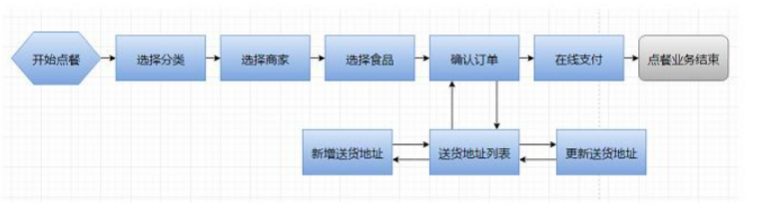
\includegraphics[width=0.8\textwidth]{servlet}
	\caption{servlet}
	\vspace{\baselineskip}
\end{figure}

\subsection{数据设计}
\subsubsection{实体类}

Business(商家)

私有变量: 

商家ID:businessId(Integer)  商家名称:businessName(String)  密码:password(String)  

商家地址:businessAddress(String)  商家描述信息:businessExplain(String)  起送费:starPrice(Double)  

配送费:deliveryPrice(Double)  商家图片:businessImg(String)  商家类别:orderTypeId(Integer)  备注:remakrs(String))



Food(商品) 

私有变量:

商品ID:foodId(Integer)  商品名:foodName(String)  商品描述信息:foodExplain(String)  价格:price(Double)  

所属商家ID:businessId(Integer)  备注:remakrs(String)  商品图片:foodImg(String))



User(用户)

私有变量:

用户ID:userId(String)  用户名:userName(String)  密码:password(String)  性别:userSex(Integer)

用户头像:userImg(String)  删除标志:delTag(Integer))



Cart(购物车订单)

私有变量:

购物车订单Id:cartId(Integer)  商家ID:businessId(Integer)  商品ID:foodId(Integer)  

用户ID:userId(String)  订购份数:quantity(Double))



DeliveryAddress(配送地址)

私有变量:

地址ID:daId(Integer)  联系人姓名:contactName(String)  联系人性别:contactSex(Integer)


联系人电话:contactTel  地址:address(String)  用户ID:userId(String))



Orders(订单)

私有变量:

订单Id:orderId(Integer)  用户ID:userId(String)  商家ID:businessId(Integer)


订单日期:orderDate(String)  订单金额:orderTotal(Double)  配送地址ID:daId(Integer)  订单状态:orderState(Integer))



OrderDetailet(订单明细)

私有变量:

订单明细ID:odId(Integer)  订单Id:orderId(Integer)  商品ID:foodId(Integer)  订单总量:quantity(Integer))

\subsubsection{工具类}
DBUtil(数据库连接工具):私有静态变量:DataSource(连接池工具,用来实现数据库持久连接)

CommonUtil(获取时间工具)
\subsection{数据库设计}

\subsubsection{business表}
    \begin{tabular}{c|c|c}
        \hline
        字段 & 类型 & 说明 \\
        \hline
        businessId & INT & 商家ID \\
        \hline
        businessName & varchar & 商家名 \\
        \hline
        password & varchar & 密码 \\
        \hline
        businessAddress & varchar & 商家地址 \\
        \hline
        businessExplain & varchar & 商家描述信息 \\
        \hline
        deliveryPrice & decimal & 配送费 \\
        \hline
        starPrice & decimal & 起送费 \\
        \hline
        orderTypeId & int & 点餐分类 \\
        \hline
        remarks & varchar & 备注 \\
    \end{tabular}

\subsubsection{food表}
    \begin{tabular}{c|c|c}
        \hline
        字段 & 类型 & 说明 \\
        \hline
        foodId & int & 商品ID \\
        \hline
        businessId & int & 所属商家ID \\
        \hline
        foodName & varchar & 商品名 \\
        \hline
        foodExplain & varchar & 商品描述信息 \\
        \hline
        foodPrice & decimal & 商品价格 \\
        \hline
        foodImg & mediumtext & 商品图片 \\
        \hline
        remakrs & varcahr & 备注 \\
    \end{tabular}
    
\subsubsection{cart表}
\begin{tabular}{c|c|c}
	\hline
	字段 & 类型 & 说明 \\
	\hline
	cartId & int & 主键,购物车编号 \\
	\hline
	foodId & int & 商品ID \\
	\hline
	businessId & int & 所属商家ID \\
	\hline
	userId & varchar & 所属用户编号 \\
	\hline
	quantity & int & 同一食品购买数量 \\
\end{tabular}

\subsubsection{deliveryaddress表}
\begin{tabular}{c|c|c}
	\hline
	字段 & 类型 & 说明 \\
	\hline
	daId & int & 主键,地址编号 \\
	\hline
	contactName & varchar & 联系人姓名 \\
	\hline
	contactSex & int & 联系人性别 \\
	\hline
	contactTel & varchar & 联系人电话 \\
	\hline
	address & varchar & 配送地址 \\
	\hline
	userId & varchar & 所属用户编号 \\
\end{tabular}

\subsubsection{orders表}
\begin{tabular}{c|c|c}
	\hline
	字段 & 类型 & 说明 \\
	\hline
	orderId & int & 主键,订单编号 \\
	\hline
	daId & int & 配送地址ID \\
	\hline
	businessId & int & 所属商家ID \\
	\hline
	userId & varchar & 所属用户编号 \\
	\hline
	orderDate & varchar & 订单日期 \\
	\hline
	orderTotal & decimal & 订单总价 \\
	\hline
	orderState & int & 订单状态 \\
\end{tabular}


\subsubsection{orderdetailet表}
\begin{tabular}{c|c|c}
	\hline
	字段 & 类型 & 说明 \\
	\hline
	odId & int & 主键,订单明细编号 \\
	\hline
	orderId & int &订单编号 \\
	\hline
	foodId & int & 商品ID \\
	\hline
	quantity & int & 数量 \\
\end{tabular}


\subsubsection{user表}
\begin{tabular}{c|c|c}
	\hline
	字段 & 类型 & 说明 \\
	\hline
	userId& varchar & 主键,用户ID \\
	\hline
	password & varchar & 密码 \\
	\hline
	userName & varchar & 用户名 \\
	\hline
	userSex & int & 性别 \\
	\hline
	userImg & mediumtext & 用户头像 \\
	\hline
	delTag & int & 删除标记 \\
\end{tabular}
\subsection{程序结构}
项目三采用的MVC架构方式。

View:该模块是是负责与用户进行交互,向服务器发送用户请求,向用户发送服务器的回复。该层主要由前端部分完成。

Controller:该模块是将前前端发送的HTTP请求进行解析拆分,操作后端程序完成正确的相对应的操作。同时打包后端返回的消息成HTTP回复发送给前端。

Model:该模块是进行数据存储和数据库操作的部分。接受Controller发送的指令,对数据库进行相对应的操作,同时向Controler返回对应的消息。

\subsection{后端模块结构划分}
\subsubsection{Controller}
DispatcherServlet:处理前端发送过来的请求,将消息解析拆分发送给对应控制器的对应方法。也接收对应Controller发回的response,将它发回给前端。

Controller:接收前端控制器(DispatcherServlet)发来的请求,将其交付给Model模块处理请求,并接受Model发回的信息发回给DispatcherServlet。

\subsubsection{Model}
Service:被Controller层调用,并调用相对应的Dao层对数据库的操作方法,将相关信息发回给Controller。

Dao:对数据库进行相关操作,返回对应信息的层。

DB:后台数据库。

\subsection{结构图}

\begin{figure}[htbp]
	\centering
	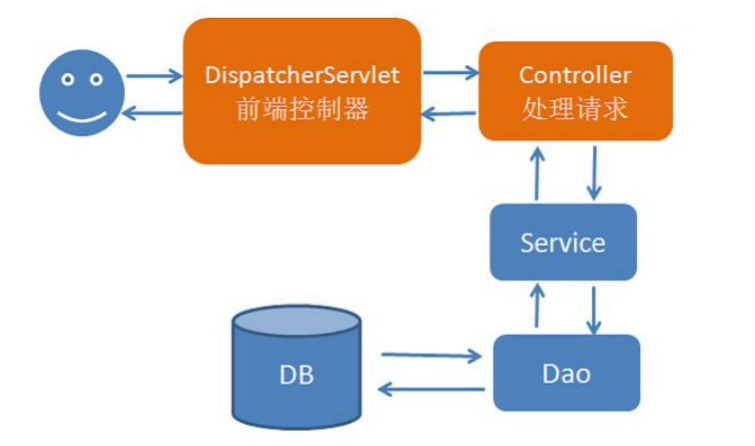
\includegraphics[width=0.8\textwidth]{MVC}
	\caption{MVC}\label{fig:MVC}
	\vspace{\baselineskip}
\end{figure}

\subsection{操作数据库接口描述}

\subsubsection{Admin}
\textbf{获取管理员对象}

getAdminByNameByPass

参数:adminName(String),password(String)

返回值:Admin

功能:传入管理员用户名和密码查找并返回对应的管理员实体。

\subsubsection{Business}
\textbf{列出相关商品类别的商家}

listBusinessByOrderTypeID

参数:orderTypeID(Integer)

返回值:List<Business>

功能:通过传入的商品类别列出此类别商家

\textbf{根据名搜索商家}

listBusinessByName

参数:businessName(String)

返回值:List<Business>

功能:通过输入字符串将商家名中含此字符串的商家列出

\textbf{根据地址搜索商家}

listBusinessByAddress

参数:businessAddress(String)

返回值:List<Business>

功能:通过输入字符串将商家字符串中含此字符串的商家列出

\textbf{获取商家}

getBusinessById

参数:businessId(Integer)

返回值:Business

功能:通过商家ID返回商家

\subsubsection{Food}
\textbf{列出商家商品}

listFoodByBusinessId

参数:businessId(Integer)

返回值:List<Food>

功能:查询数据库,列出商家ID对应商家的商品列表

\subsubsection{User}
\textbf{根据ID和密码返回账户}

getUserByIdByPass

参数:userId(String),password(String)

返回值:User

功能:根据输入的ID和密码返回对应账户

\textbf{查询账户}

getUserById

参数:userId(String)

返回值:int

功能:根据ID查询用户是否存在

\textbf{注册用户}

saveUser

参数:user(User)

返回值:int

功能:将传入的用户存入数据库

\textbf{更新用户名}

updateUserMsg

参数:userId(String),userName(String)

返回值:int

功能:修改对应ID的用户的用户名

\textbf{更新用户密码}

updateUserPassword

参数:userId(String),oldPass(String),newPass(String)

返回值:int

功能:判断密码是否正确。如果正确修改对应ID的用户的密码

\subsubsection{Cart}
\textbf{新建购物车账单}

saveCart

参数:cart(Cart)

返回值:int

功能:将传入的购物车账单存入数据库

\textbf{更新购物车}

updateCart

参数:cart(Cart)

返回值:int

功能:将与传入的购物车ID相同的购物车账单信息更新

\textbf{删除购物车账单}

removeCart

参数:cart(Cart)

返回值:int

功能:将与传入的购物车ID相同的购物车账单在数据库中删除

\textbf{列出购物车清单}

removeCart

参数:cart(Cart)

返回值:int

功能:如果存在businessId,列出对应user在此商家的购物车订单;如果不存在,列出此user所有的购物车账单

\subsubsection{DeliveryAddress}

\textbf{列出用户配送地址}

listDeliveryAddressByUserId

参数:userId(String)

返回值:List<DeliveryAddress>

功能:列出ID对应user的所有配送地址

\textbf{列出用户配送地址}

saveDeliveryAddress

参数:deliveryAddress(DeliveryAddress)

返回值:int

功能:将传入的地址存入数据库

\textbf{列出用户配送地址}

updateDeliveryAddress

参数:deliveryAddress(DeliveryAddress)

返回值:int

功能:将数据库中与传入参数daId相同的配送地址信息更新


\textbf{列出用户配送地址}

updateDeliveryAddress

参数:removeDeliveryAddress(DeliveryAddress)

返回值:int

功能:将数据库中与传入参数daId相同的配送地址删除

\textbf{根据地址ID查询地址}

getDeliveryAddressById

参数:daId(Integer)

返回值:DeliveryAddress

功能:将数据库中查询传对应daId的地址

\subsubsection{Orders}

\textbf{新建订单}

saveOrders

参数:orders(Orders)

返回值:int

功能:向数据库中存入传入的订单

\textbf{查询订单}

getOrdersById

参数:orderId(Integer)

返回值:Orders

功能:查询出与传入orderId相等的订单

\textbf{查询订单}

listOrdersByUserId

参数:userId(String)

返回值:List<Orders>

功能:列出与userId对应的用户的所有订单

\subsubsection{OrderDetailet}

\textbf{存储订单明细}

saveOrderDetailetBatch

参数:list(List<OrderDetailet>) 

返回值:int

功能:将传入的订单明细组存入数据库

\textbf{存储订单明细}

listOrderDetailetByOrderId

参数:orderId(Integer) 

返回值:List<OrderDetailet>

功能:列出所有数据库中与传入orderId相同的订单明细

\subsection{对外接口}
\textbf{处理http get方法}

DispatcherServlet/doGet

参数:request(HttpServletRequest) ,response(HttpServletResponse)

返回值:void

功能:处理发送的HTTP请求,将其发送给对应的Controller,让后端进行对应数据库操作,并将返回消息封装进response

\textbf{处理http Post方法}

DispatcherServlet/doPost

参数:request(HttpServletRequest) ,response(HttpServletResponse)

返回值:void

功能:处理发送的HTTP请求,将其发送给对应的Controller,让后端进行对应数据库操作,并将返回消息封装进response

\section{测试}
\subsection{测试中问题}
Invalid value for getInt()
\section{部署}